% options:
% thesis=B bachelor's thesis
% thesis=M master's thesis
% czech thesis in Czech language
% slovak thesis in Slovak language
% english thesis in English language
% hidelinks remove colour boxes around hyperlinks

\documentclass[thesis=B,czech]{FITthesis}[2013/05/06]

\usepackage[utf8]{inputenc} % LaTeX source encoded as UTF-8

\usepackage{graphicx} %graphics files inclusion
% \usepackage{amsmath} %advanced maths
% \usepackage{amssymb} %additional math symbols

\usepackage{dirtree} %directory tree visualisation

% % list of acronyms
% \usepackage[acronym,nonumberlist,toc,numberedsection=autolabel]{glossaries}
% \iflanguage{czech}{\renewcommand*{\acronymname}{Seznam pou{\v z}it{\' y}ch zkratek}}{}
% \makeglossaries

\newcommand{\tg}{\mathop{\mathrm{tg}}} %cesky tangens
\newcommand{\cotg}{\mathop{\mathrm{cotg}}} %cesky cotangens

% % % % % % % % % % % % % % % % % % % % % % % % % % % % % %
% ODTUD DAL VSE ZMENTE
% % % % % % % % % % % % % % % % % % % % % % % % % % % % % %

\department{Katedra softwarového inženýrství}
\title{Kolaborativní tvorba LaTeX dokumentů s podporou Gitu}
\authorGN{Filip} %(křestní) jméno (jména) autora
\authorFN{Chalupa} %příjmení autora
\authorWithDegrees{Filip Chalupa} %jméno autora včetně současných akademických titulů
\supervisor{Ing. Tomáš Kalvoda, Ph.D.}
\acknowledgements{Doplňte, máte-li komu a za co děkovat. V~opačném případě úplně odstraňte tento příkaz.}
\abstractCS{V~několika větách shrňte obsah a přínos této práce v~češtině. Po přečtení abstraktu by se čtenář měl mít čtenář dost informací pro rozhodnutí, zda chce Vaši práci číst.}
\abstractEN{Sem doplňte ekvivalent abstraktu Vaší práce v~angličtině.}
\placeForDeclarationOfAuthenticity{V~Praze}
\declarationOfAuthenticityOption{4} %volba Prohlášení (číslo 1-6)
\keywordsCS{LaTeX, Git, verzování, kolaborace, přístupnost}
\keywordsEN{LaTeX, Git, versioning, collaboration, accessibility}

\begin{document}

% \newacronym{CVUT}{{\v C}VUT}{{\v C}esk{\' e} vysok{\' e} u{\v c}en{\' i} technick{\' e} v Praze}
% \newacronym{FIT}{FIT}{Fakulta informa{\v c}n{\' i}ch technologi{\' i}}

\chapter{Úvod}
Častým scénářem při tvorbě různých skript, vědeckých článků, informačních podkladů, prezentací je spolupráce několika osob. V takových týmech je důležitá komunikace mezi jednotlivými členy a sdílení aktuálního rozpracovaného díla.

\section{Hypotéza}

K dispozici je spousta nástrojů, jejichž smyslem je tvorbu ve skupině usnadnit; velké množství, různorodost, a v některých případech větší komplexita však značně komplikuje jejich nasazení. Důsledkem je uchýlení se k více známým a z podstaty primitivnějším řešením, například přeposílání rozdělané práce přes e-mail nebo předávání podkladů přes externí uložiště a nedělání záloh předešlých verzí. Tým tím ztrácí na efektivitě, což se může podepsat na kvalitě díla a zbytečném protahování tvorby.

\section{Terminologie}

\subsection{\LaTeX}

\uv{LaTeX je komplexní systém pro sazbu dokumentů. Stará se tedy o zalamování textu do odstavců, vkládání obrázků, seznamů, nadpisů, matematických výrazů, rozdělování dokumentu na jednotlivé stránky, ligatury, "vdovy" a "sirotky", odsazení\ldots} \cite{latex-def}

\subsection{Git}

Verzovací systém s podporou více uživatelů a ukládáním projektu na vzdálený server například v internetu.

\subsection{Verzování}

Sledování projektu s průběžným ukládání změn pro zpětné dohledání přidaných či odebraných řádků v textovém souboru, případně přidání či odebrání binárního souboru.

\subsection{Kolaborace}

Spolupráce více osob na jednom projektu.

\subsection{Přístupnost}

Umožnění práce se složitějšími nástroji pro osoby s nedostatečnou znalostí ovládání.

\section{Struktura práce}

Následující kapitoly se budou zabývat ověřením hypotézy pomocí uživatelského průzkumu a analýzou existujících řešení, návrhem vlastního řešení s požadavky a volbou prostředků pro jeho implementaci, podrobnějším rozborem tvorby uživatelského rozhraní, distribucí aplikace, testováním, poznatky ohledně knihovny NodeGit, návrhy na další vývoj a závěrečným shrnutím.


\chapter{Cíl práce}
Tristní situaci přednesenou v úvodu je tedy žádoucí vyřešit buď vyškolením účastníků týmu, nebo představením nového nástroje, který disponuje funkcemi komplexních nástrojů, ale zároveň je jednoduchý na použití i pro začátečníka, což je i cílem této práce, zhotovení nové aplikace určené pro operační systémy primárně Windows a Linux. K jeho dosažení je potřeba provést podrobnější analýzu současného stavu. Je tedy nutné proniknout do pracovních postupů autorů, jimž práce v týmu psaním v LaTeXu způsobuje potíže. Na základě například dotazníků či rozhovorů. Tímto se dostaneme do druhé fáze, kdy bude potřeba navrhnout principy aplikace, její nároky na uživatelské rozhraní a podporované funkce. Dále dojde k implementaci vybraného návrhu a na závěr k otestovaní dotazovanými z analytické části.


\chapter{Současný stav}
Jako ověření, že vytváření nové aplikace má význam, byly prozkoumány současné možnosti, které si kladou za cíl řešení stejného problému. K dispozici jsou například online nástroje ShareLaTeX a Overleaf. První zmíněný, „Online LaTeX editor snadný k použití s možností spolupráce více autorů“ {cit2}, se sice hned na úvodní stránce chlubí překladem do češtiny, který je ale nekompletní a práce s ním je tak často matoucí, z textů není jasné, co se zrovna děje, co se od uživatele očekává a jakým způsobem má pracovat. K tomu vyžaduje vysoký měsíční poplatek {cit3} za zpřístupnění většiny funkcí. Druhá služba, Overleaf, překlad do češtiny nenabízí vůbec, což není nutné považovat za nedostatek, protože požadavkem není řešení konkrétně pro české prostředí. Chybí však funkce pro procházení změn v historii projektu.

Obě služby trpí omezením, že se nelze dostat k úpravám projektu mimo ně. Uživatel nemůže tvořit ve svém oblíbeném editoru, musí si vystačit s online editorem, který navíc nenabízí žádnou offline variantu.

Alternativním přístupem je třeba verzovací systém Git, jež je zejména pro začátečníky s tímto systémem příliš komplikovaný.

těm psům


\chapter{Řešení}
Řešením je nová aplikace, která je schopná běžet na různých cílových zařízení, se systémem Windows nebo Linux, tak, aby vystihla různorodost zařízení členů týmu (systém, editor LaTeXu), ale zároveň nenutila všechny členy k jejímu aktivnímu využívání. Čtyřčlenný tým může vypadat třeba tak, že jeden autor pracuje na svém počítači se systémem Windows s pomocí nové aplikace, podobně další dva členové se systémem Linux a čtvrtý člen s pokročilou znalostí verzovacího systému Git nemusí novou aplikaci používat vůbec a stejně může bez omezení spolupracovat se zbytkem týmu. Aplikace tedy musí být schopná komunikovat se systémem Git, který splňuje požadavek na zálohování a verzování.


\chapter{Realizace}

\begin{conclusion}
	%sem napište závěr Vaší práce
	Bakalářská práce je momentálně již rozpracovaná. Byl proveden průzkum mezi šesti učiteli, kteří v LaTeXu běžně tvoří obsah v týmu. V rozhovorech se všichni shodli, že aktuální stav není ideální a až na jednoho člověka by všichni ocenili lepší, přehlednější řešení. Mimo to byly také prozkoumány alternativní nástroje, které jsou ve spojení LaTeXu a spolupráce známé, ale nikdo z tázaných s nimi neměl zkušenost. Konkrétně se jednalo o webové služby ShareLaTeX [2] a Overleaf {cit4}. Závěrem je potvrzení, že má smysl nové řešení vyvíjet a zároveň došlo k jeho detailnější specifikaci.
\end{conclusion}

\bibliographystyle{csn690}
\bibliography{mybibliographyfile}

\appendix

\chapter{Seznam použitých zkratek}
% \printglossaries
\begin{description}
	\item[GUI] Graphical user interface
	\item[XML] Extensible markup language
\end{description}


% % % % % % % % % % % % % % % % % % % % % % % % % % % %
% % Tuto kapitolu z výsledné práce ODSTRAŇTE.
% % % % % % % % % % % % % % % % % % % % % % % % % % % %
%
% \chapter{Návod k~použití této šablony}
%
% Tento dokument slouží jako základ pro napsání závěrečné práce na Fakultě informačních technologií ČVUT v~Praze.
%
% \section{Výběr základu}
%
% Vyberte si šablonu podle druhu práce (bakalářská, diplomová), jazyka (čeština, angličtina) a kódování (ASCII, \mbox{UTF-8}, \mbox{ISO-8859-2} neboli latin2 a nebo \mbox{Windows-1250}).
%
% V~české variantě naleznete šablony v~souborech pojmenovaných ve formátu práce\_kódování.tex. Typ může být:
% \begin{description}
% 	\item[BP] bakalářská práce,
% 	\item[DP] diplomová (magisterská) práce.
% \end{description}
% Kódování, ve kterém chcete psát, může být:
% \begin{description}
% 	\item[UTF-8] kódování Unicode,
% 	\item[ISO-8859-2] latin2,
% 	\item[Windows-1250] znaková sada 1250 Windows.
% \end{description}
% V~případě nejistoty ohledně kódování doporučujeme následující postup:
% \begin{enumerate}
% 	\item Otevřete šablony pro kódování UTF-8 v~editoru prostého textu, který chcete pro psaní práce použít -- pokud můžete texty s~diakritikou normálně přečíst, použijte tuto šablonu.
% 	\item V~opačném případě postupujte dále podle toho, jaký operační systém používáte:
% 	\begin{itemize}
% 		\item v~případě Windows použijte šablonu pro kódování \mbox{Windows-1250},
% 		\item jinak zkuste použít šablonu pro kódování \mbox{ISO-8859-2}.
% 	\end{itemize}
% \end{enumerate}
%
%
% V~anglické variantě jsou šablony pojmenované podle typu práce, možnosti jsou:
% \begin{description}
% 	\item[bachelors] bakalářská práce,
% 	\item[masters] diplomová (magisterská) práce.
% \end{description}
%
% \section{Použití šablony}
%
% Šablona je určena pro zpracování systémem \LaTeXe{}. Text je možné psát v~textovém editoru jako prostý text, lze však také využít specializovaný editor pro \LaTeX{}, např. Kile.
%
% Pro získání tisknutelného výstupu z~takto vytvořeného souboru použijte příkaz \verb|pdflatex|, kterému předáte cestu k~souboru jako parametr. Vhodný editor pro \LaTeX{} toto udělá za Vás. \verb|pdfcslatex| ani \verb|cslatex| \emph{nebudou} s~těmito šablonami fungovat.
%
% Více informací o~použití systému \LaTeX{} najdete např. v~\cite{wikilatex}.
%
% \subsection{Typografie}
%
% Při psaní dodržujte typografické konvence zvoleného jazyka. České \uv{uvozovky} zapisujte použitím příkazu \verb|\uv|, kterému v~parametru předáte text, jenž má být v~uvozovkách. Anglické otevírací uvozovky se v~\LaTeX{}u zadávají jako dva zpětné apostrofy, uzavírací uvozovky jako dva apostrofy. Často chybně uváděný symbol "{} (palce) nemá s~uvozovkami nic společného.
%
% Dále je třeba zabránit zalomení řádky mezi některými slovy, v~češtině např. za jednopísmennými předložkami a spojkami (vyjma \uv{a}). To docílíte vložením pružné nezalomitelné mezery -- znakem \texttt{\textasciitilde}. V~tomto případě to není třeba dělat ručně, lze použít program \verb|vlna|.
%
% Více o~typografii viz \cite{kobltypo}.
%
% \subsection{Obrázky}
%
% Pro umožnění vkládání obrázků je vhodné použít balíček \verb|graphicx|, samotné vložení se provede příkazem \verb|\includegraphics|. Takto je možné vkládat obrázky ve formátu PDF, PNG a JPEG jestliže používáte pdf\LaTeX{} nebo ve formátu EPS jestliže používáte \LaTeX{}. Doporučujeme preferovat vektorové obrázky před rastrovými (vyjma fotografií).
%
% \subsubsection{Získání vhodného formátu}
%
% Pro získání vektorových formátů PDF nebo EPS z~jiných lze použít některý z~vektorových grafických editorů. Pro převod rastrového obrázku na vektorový lze použít rasterizaci, kterou mnohé editory zvládají (např. Inkscape). Pro konverze lze použít též nástroje pro dávkové zpracování běžně dodávané s~\LaTeX{}em, např. \verb|epstopdf|.
%
% \subsubsection{Plovoucí prostředí}
%
% Příkazem \verb|\includegraphics| lze obrázky vkládat přímo, doporučujeme však použít plovoucí prostředí, konkrétně \verb|figure|. Například obrázek \ref{fig:float} byl vložen tímto způsobem. Vůbec přitom nevadí, když je obrázek umístěn jinde, než bylo původně zamýšleno -- je tomu tak hlavně kvůli dodržení typografických konvencí. Namísto vynucování konkrétní pozice obrázku doporučujeme používat odkazování z~textu (dvojice příkazů \verb|\label| a \verb|\ref|).
%
% \begin{figure}\centering
% 	
\includegraphics[width=0.5\textwidth, angle=30]{cvut-logo-bw}
% 	\caption[Příklad obrázku]{Ukázkový obrázek v~plovoucím prostředí}\label{fig:float}
% \end{figure}
%
% \subsubsection{Verze obrázků}
%
% % Gnuplot BW i barevně
% Může se hodit mít více verzí stejného obrázku, např. pro barevný či černobílý tisk a nebo pro prezentaci. S~pomocí některých nástrojů na generování grafiky je to snadné.
%
% Máte-li například graf vytvořený v programu Gnuplot, můžete jeho černobílou variantu (viz obr. \ref{fig:gnuplot-bw}) vytvořit parametrem \verb|monochrome dashed| příkazu \verb|set term|. Barevnou variantu (viz obr. \ref{fig:gnuplot-col}) vhodnou na prezentace lze vytvořit parametrem \verb|colour solid|.
%
% \begin{figure}\centering
% 	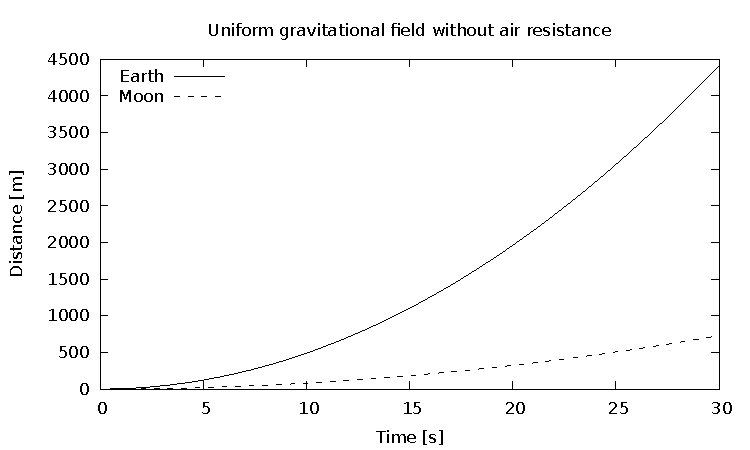
\includegraphics{gnuplot-bw}
% 	\caption{Černobílá varianta obrázku generovaného programem Gnuplot}\label{fig:gnuplot-bw}
% \end{figure}
%
% \begin{figure}\centering
% 	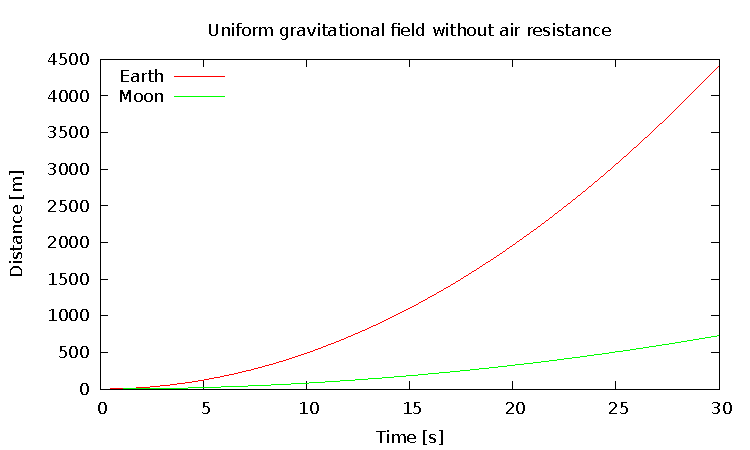
\includegraphics{gnuplot-col}
% 	\caption{Barevná varianta obrázku generovaného programem Gnuplot}\label{fig:gnuplot-col}
% \end{figure}
%
%
% \subsection{Tabulky}
%
% Tabulky lze zadávat různě, např. v~prostředí \verb|tabular|, avšak pro jejich vkládání platí to samé, co pro obrázky -- použijte plovoucí prostředí, v~tomto případě \verb|table|. Například tabulka \ref{tab:matematika} byla vložena tímto způsobem.
%
% \begin{table}\centering
% 	\caption[Příklad tabulky]{Zadávání matematiky}\label{tab:matematika}
% 	\begin{tabular}{|l|l|c|c|}\hline
% 		Typ		& Prostředí		& \LaTeX{}ovská zkratka	& \TeX{}ovská zkratka	\tabularnewline \hline \hline
% 		Text		& \verb|math|		& \verb|\(...\)|	& \verb|$...$|		\tabularnewline \hline
% 		Displayed	& \verb|displaymath|	& \verb|\[...\]|	& \verb|$$...$$|	\tabularnewline \hline
% 	\end{tabular}
% \end{table}
%
% % % % % % % % % % % % % % % % % % % % % % % % % % % %

\chapter{Obsah přiloženého CD}

%upravte podle skutecnosti

\begin{figure}
	\dirtree{%
		.1 readme.txt\DTcomment{stručný popis obsahu CD}.
		.1 exe\DTcomment{adresář se spustitelnou formou implementace}.
		.1 src.
		.2 impl\DTcomment{zdrojové kódy implementace}.
		.2 thesis\DTcomment{zdrojová forma práce ve formátu \LaTeX{}}.
		.1 text\DTcomment{text práce}.
		.2 thesis.pdf\DTcomment{text práce ve formátu PDF}.
		.2 thesis.ps\DTcomment{text práce ve formátu PS}.
	}
\end{figure}

\end{document}
